\documentclass[presentation,aspectratio=169]{ctexbeamer}

%\setbeameroption{show notes}
%\setbeameroption{show notes on second screen=right}

%\setbeamertemplate{footline} % To remove the footer line in all slides uncomment this line
\setbeamertemplate{sidebar left}[frame number]
\hypersetup{pdfpagemode=FullScreen} % fullscreen mode
%\setbeamertemplate{navigation symbols}{} % To remove the navigation symbols from the bottom of all slides uncomment this line
\usetheme{SCUT}

%----------------------------------------------------------------------------------------
%	TITLE PAGE
%----------------------------------------------------------------------------------------

\title{毕业设计} % The short title appears at the bottom of every slide, the full title is only on the title page
\subtitle{基于稀疏性优化的卡尔曼滤波状态转移模型参数估计}
\author{邓肯} % Your name
\institute % Your institution as it will appear on the bottom of every slide, may be shorthand to save space
{
数学学院 \\ % Your institution for the title page
\medskip
202130320311@mail.scut.edu.cn % Your email address
}
\date{\today} % Date, can be changed to a custom date

\begin{document}

\begin{frame}
\titlepage % Print the title page as the first slide
\end{frame}

\begin{frame}
\frametitle{Overview} % Table of contents slide, comment this block out to remove it
\tableofcontents % Throughout your presentation, if you choose to use \section{} and \subsection{} commands, these will automatically be printed on this slide as an overview of your presentation
\end{frame}

%----------------------------------------------------------------------------------------
%	PRESENTATION SLIDES
%----------------------------------------------------------------------------------------

\section{研究背景}

\begin{frame}
\Huge{\centerline{\textcolor{covblue}{研究背景}}}
\end{frame}

\begin{frame}{问题背景}
状态空间模型 (SSM) 广泛应用于工程~\cite{hamilton1994state, kim2017state}、环境科学~\cite{choi2023urban_phd_environ}、信号处理~\cite{dabush2024kalman_tracking_network_dynamic} 等各个领域的随机过程建模。SSM 利用隐藏变量来表示底层的马尔可夫过程,使其成为分析时间序列数据的强大工具。
\vspace{8pt}
\pause

当模型参数已知时,贝叶斯最优滤波器和平滑器为求解状态空间模型~\cite{Särkkä_Svensson_2023_textbook} 提供了理论框架。这些工具能够进行准确的预测,为工业应用中的决策和战略制定提供参考。具体而言,贝叶斯滤波器能够以高可靠性预测状态空间模型中的长期行为。在线性高斯状态空间模型 (LGSSM) 中,该过程允许一个解析解,详见~\cite{Särkkä_Svensson_2023_textbook}。对于非线性状态空间模型,粒子滤波器提供了一种实用的解决方案。
\vspace{8pt}
\pause

本文重点介绍线性高斯状态空间模型 (LGSSM)。在 LGSSM 中,诸如转移矩阵之类的参数对于理解卡尔曼滤波器的行为至关重要。转移矩阵封装了不同的马尔可夫链,其准确估计至关重要。然而,在实际场景中,模型参数通常未知,但具有特定的属性~\cite{watts1998collective},因此模型的参数估计是一项至关重要的任务。
\end{frame}

\section{相关文献}

\begin{frame}
\Huge{\centerline{\textcolor{covblue}{相关文献}}}
\end{frame}

\begin{frame}{相关文献}
卡尔曼滤波器及其扩展的理论基础已非常完善,~\cite{Särkkä_Svensson_2023_textbook}提供了全面的推导和分析。
\vspace{8pt}

卡尔曼滤波器的参数估计已得到广泛研究,其中期望最大化 (EM) 算法是最广泛使用的方法之一。EM 算法(如~\cite{Särkkä_Svensson_2023_textbook} 所述)通过迭代优化似然函数,为估计模型参数提供了一个稳健的框架。然而,传统的 EM 方法通常缺乏融入先验知识的能力,而这对于提高实际应用中的估计精度至关重要。
\vspace{8pt}
\pause

与此同时,其他研究人员也在探索状态空间模型中参数估计的替代方法。例如,~\cite{tsampourakis2022alr_changepoint} 提出了一种用于变点检测的自适应调优方法,而~\cite{sharma2023stock_later} 将 GraphEM 与循环神经网络 (RNN) 相结合,用于股票市场预测。此外,~\cite{cui2024inference_non_linear} 使用哈密顿蒙特卡罗方法研究了非线性系统的推理方法,~\cite{mohanty2025iclr_granger} 则在图模型的背景下探索了格兰杰因果关系。
\end{frame}

% \begin{frame}{相关文献}
% GraphEM 的进一步扩展已在时间序列预测和非凸优化领域得到探索。例如,~\cite{elvira2022GraphEM_TSP} 将 GraphEM 应用于旅行商问题 (TSP) 场景,而 ~\cite{chouzenoux2023graph_it} 则研究了其在非凸设置下的性能。此外,~\cite{chouzenoux2024non_markov_lagrangeEM} 提出了一种基于拉格朗日的 GraphEM 变体,用于非马尔可夫系统,进一步拓宽了其适用性。
% \vspace{8pt}

% 近期的研究也致力于提升 GraphEM 的计算效率和可扩展性。例如,~\cite{cox2022sparj_alg_journal} 引入了 SPARJ 算法,提高了大规模系统中图推理的效率。该算法在 ~\cite{cox2023sparj_alg} 和 ~\cite{cox2024graphgrad_TSP} 中得到了进一步扩展,其中集成了基于梯度的方法来处理高维转移矩阵。此外,~\cite{chouzenoux2024DGLASSO} 提出了一种联合估计转移矩阵和噪声协方差的新方法,显著提高了估计精度。
% \vspace{8pt}


% \end{frame}

\section{研究方法}

\begin{frame}
\Huge{\centerline{\textcolor{covblue}{研究方法}}}
\end{frame}

\begin{frame}{线性高斯状态空间模型}
卡尔曼滤波器是贝叶斯滤波器的一个特例,其中动态模型和测量模型均为线性高斯模型。该模型由以下方程定义:
\begin{align}
\mathbf{x}_k &= \mathbf{A}_{k-1} \mathbf{x}_{k-1} + \mathbf{q}_{k-1}, \\
\mathbf{y}_k &= \mathbf{H}_k \mathbf{x}_k + \mathbf{r}_k,
\end{align}
\pause
其中:
\begin{itemize}
\item \(\mathbf{q}_{k-1} \sim \mathcal{N}(\mathbf{0}, \mathbf{Q}_{k-1})\) 是过程噪声,假设为具有零均值和协方差的高斯分布\(\mathbf{Q}_{k-1}\),
\item \(\mathbf{r}_k \sim \mathcal{N}(\mathbf{0}, \mathbf{R}_k)\) 为测量噪声,假设为均值为零、协方差为 \(\mathbf{R}_k\) 的高斯分布。
\item \(\mathbf{x}_0 \sim \mathcal{N}(\mathbf{m}_0, \mathbf{P}_0)\) 为初始状态,假设为均值为 \(\mathbf{m}_0\)、协方差为 \(\mathbf{P}_0\) 的高斯分布。
\item \(\mathbf{A}_{k-1}\) 为状态转移矩阵。
\item \(\mathbf{H}_k\) 是观测矩阵。
\end{itemize}
\end{frame}

\begin{frame}
\begin{figure}[tb]
\centering
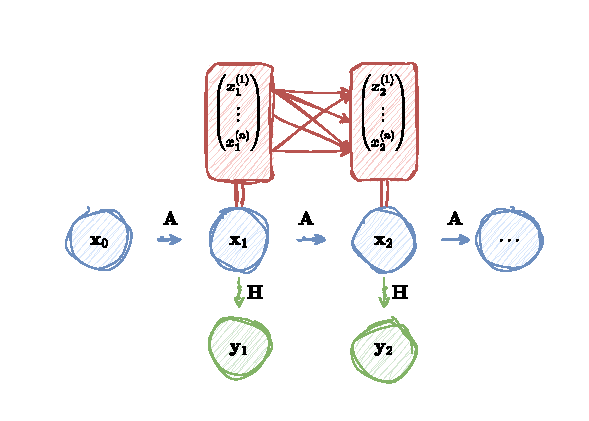
\includegraphics[width=0.75\linewidth]{fig/Markov Chian.pdf}
\caption{\textit{线性高斯状态空间模型}的流程。\textcolor{blue}{蓝色块}表示\textit{转换过程},\textcolor{red}{红色块}说明\textit{马尔可夫链属性}的细节,\textcolor{green}{绿色块}表示\textit{观察过程}。}
\label{fig: LGSSM 流程图}
\end{figure}
\end{frame}

\begin{frame}{具有缺失参数的线性高斯状态空间模型}
具有缺失参数 \(\boldsymbol{\theta}\) 的线性高斯状态空间模型(LGSSM)定义为:
\begin{align}
    \mathbf{x}_k &= \mathbf{A}(\boldsymbol{\theta}) \, \mathbf{x}_{k-1} + \mathbf{q}_{k-1}, \\
    \mathbf{y}_k &= \mathbf{H}(\boldsymbol{\theta}) \, \mathbf{x}_k + \mathbf{r}_k,
\end{align}
\pause
其中:
\begin{itemize}
    \item \(\mathbf{q}_{k-1} \sim \mathcal{N}(\mathbf{0}, \mathbf{Q}(\boldsymbol{\theta}))\) 和 \(\mathbf{r}_{k} \sim \mathcal{N}(\mathbf{0}, \mathbf{R}(\boldsymbol{\theta}))\) 分别是过程噪声和测量噪声,
    \item \(\mathbf{x}_0 \sim \mathcal{N}(\mathbf{m}_0(\boldsymbol{\theta}), \mathbf{P}_0(\boldsymbol{\theta}))\) 是初始状态分布,
    \item 假设模型参数 \(\boldsymbol{\theta}\) 是时间不变的。
\end{itemize}
\end{frame}

\begin{frame}{简略EM算法}
令 \(q(\mathbf{x}_{0:T})\) 为状态 \(\mathbf{x}_{0:T}\) 上的任意概率密度函数。对于对数似然 \(\log p(\mathbf{y}_{1:T} \mid \boldsymbol{\theta})\),总是存在一个下界,如下所示:
\begin{align}
    \log p(\mathbf{y}_{1:T} \mid \boldsymbol{\theta}) \ge F(q(\mathbf{x}_{0:T}), \boldsymbol{\theta}), \label{eq: ineq for EM}
\end{align}
其中二元函数 \(F(\cdot)\) 定义为:
\begin{align}
    F(q(\mathbf{x}_{0:T}), \boldsymbol{\theta}) = \int q(\mathbf{x}_{0:T}, \boldsymbol{\theta}) \, \log \frac{p(\mathbf{x}_{0:T}, \mathbf{y}_{1:T} \mid \boldsymbol{\theta})}{q(\mathbf{x}_{0:T}, \boldsymbol{\theta})} \, \mathrm{d} \mathbf{x}_{0:T}.
\end{align}
\end{frame}

\begin{frame}{求解EM算法}
为了求解算法中的 E 步骤,我们直接给出最优解:
\begin{align}
    q^{(n+1)}(\mathbf{x}_{0:T}) &= p(\mathbf{x}_{0:T} \mid \mathbf{y}_{1:T}, \boldsymbol{\theta}^{(n)}), \\
    F[q^{(n+1)}(\mathbf{x}_{0:T}), \boldsymbol{\theta}] &= \int p(\mathbf{x}_{0:T} \mid \mathbf{y}_{1:T}, \boldsymbol{\theta}^{(n)}) \log p(\mathbf{x}_{0:T}, \mathbf{y}_{1:T} \mid \boldsymbol{\theta}) \, \mathrm{d} \mathbf{x}_{0:T} \label{eq: full lower bound} \\
    &\quad - \int p(\mathbf{x}_{0:T} \mid \mathbf{y}_{1:T}, \boldsymbol{\theta}^{(n)}) \log p(\mathbf{x}_{0:T} \mid \mathbf{y}_{1:T}, \boldsymbol{\theta}^{(n)}) \, \mathrm{d} \mathbf{x}_{0{T}}. \nonumber
\end{align}
\end{frame}

\begin{frame}{EM算法结论}
注意,方程~\eqref{eq: full lower bound} 中的第二项不依赖于 \(\boldsymbol{\theta}\)。因此,算法中的 M 步骤优化可以简化,只考虑方程~\eqref{eq: full lower bound} 中的第一项作为对数似然的新下界,记作 \(\mathcal{Q}(\boldsymbol{\theta}, \boldsymbol{\theta}^{(n)})\):
\begin{align}
\mathcal{Q}(\boldsymbol{\theta}, \boldsymbol{\theta}^{(n)}) = \int p(\mathbf{x}_{0:T} \mid \mathbf{y}_{1:T}, \boldsymbol{\theta}^{(n)}) \log p(\mathbf{x}_{0:T}, \mathbf{y}_{1:T} \mid \boldsymbol{\theta}) \, \mathrm{d} \mathbf{x}_{0:T}.
\end{align}
\pause

因此,我们得到了最终的迭代不等式,改编自方程~\eqref{eq: ineq for EM}:
\begin{align}
    \log p(\mathbf{y}_{1:T} \mid \boldsymbol{\theta}) \ge \mathcal{Q}(\boldsymbol{\theta}, \boldsymbol{\theta}^{(n)}). \label{eq: ineq for EM final}
\end{align}
\end{frame}

\begin{frame}{线性高斯状态空间模型的 EM 算法}
在线性高斯状态空间模型(LGSSM)的假设下,\(\mathcal{Q}(\boldsymbol{\theta}, \boldsymbol{\theta}^{(n)})\) 的表达式为:
\begin{align}
    \mathcal{Q}(\boldsymbol{\theta}, \boldsymbol{\theta}^{(n)}) &= -\frac{1}{2} \log |2\pi \mathbf{P}_0(\boldsymbol{\theta})| - \frac{T}{2} \log |2\pi \mathbf{Q}(\boldsymbol{\theta})| - \frac{T}{2} \log |2\pi \mathbf{R}(\boldsymbol{\theta})| \nonumber \\
    &\quad - \frac{1}{2} \mathrm{tr} \left\{ \mathbf{P}_0^{-1}(\boldsymbol{\theta}) \left[ \mathbf{P}_0^s + (\mathbf{m}_0^s - \mathbf{m}_0(\boldsymbol{\theta}))(\mathbf{m}_0^s - \mathbf{m}_0(\boldsymbol{\theta}))^\mathsf{T} \right] \right\} \nonumber \\
    &\quad - \frac{T}{2} \mathrm{tr} \left\{ \mathbf{Q}^{-1}(\boldsymbol{\theta}) \left[ \boldsymbol{\Sigma} - \mathbf{C} \mathbf{A}^\mathsf{T}(\boldsymbol{\theta}) - \mathbf{A}(\boldsymbol{\theta}) \mathbf{C}^\mathsf{T} + \mathbf{A}(\boldsymbol{\theta}) \boldsymbol{\Phi} \mathbf{A}^\mathsf{T}(\boldsymbol{\theta}) \right] \right\} \nonumber \\
    &\quad - \frac{T}{2} \mathrm{tr} \left\{ \mathbf{R}^{-1}(\boldsymbol{\theta}) \left[ \mathbf{D} - \mathbf{B} \mathbf{H}^\mathsf{T}(\boldsymbol{\theta}) - \mathbf{H}(\boldsymbol{\theta}) \mathbf{B}^\mathsf{T} + \mathbf{H}(\boldsymbol{\theta}) \boldsymbol{\Sigma} \mathbf{H}^\mathsf{T}(\boldsymbol{\theta}) \right] \right\}, \label{eq: Q for LGSSM}
\end{align}
\end{frame}

\begin{frame}
其中,中间量 \(\boldsymbol{\Sigma}, \boldsymbol{\Phi}, \mathbf{B}, \mathbf{C}, \mathbf{D}\) 计算为:
\begin{align}
    \boldsymbol{\Sigma} &= \frac{1}{T} \sum_{k=1}^{T} \mathbf{P}_k^s + \mathbf{m}_k^s [\mathbf{m}_k^s]^\mathsf{T}, \label{eq: middle Sigma} \\
    \boldsymbol{\Phi} &= \frac{1}{T} \sum_{k=1}^{T} \mathbf{P}_{k-1}^s + \mathbf{m}_{k-1}^s [\mathbf{m}_{k-1}^s]^\mathsf{T}, \label{eq: middle Phi} \\
    \mathbf{B} &= \frac{1}{T} \sum_{k=1}^{T} \mathbf{y}_k [\mathbf{m}_k^s]^\mathsf{T}, \label{eq: middle B} \\
    \mathbf{C} &= \frac{1}{T} \sum_{k=1}^{T} \mathbf{P}_k^s \mathbf{G}_{k-1}^\mathsf{T} + \mathbf{m}_k^s [\mathbf{m}_{k-1}^s]^\mathsf{T}, \label{eq: middle C} \\
    \mathbf{D} &= \frac{1}{T} \sum_{k=1}^{T} \mathbf{y}_k \mathbf{y}_k^\mathsf{T}, \label{eq: middle D}
\end{align}
这些量是由\textit{卡尔曼滤波器}和\textit{卡尔曼平滑器}的结果推导而来。
\end{frame}

\begin{frame}
通过将梯度 \(\frac{\partial \mathcal{Q} (\boldsymbol{\theta}, \boldsymbol{\theta}^{(n)})}{\partial \boldsymbol{\theta}}\) 设置为零,我们得到以下解析形式的公式来更新参数:
\begin{align}
    \mathbf{m}_0^* &= \mathbf{m}_0^s, \label{eq: EM-M m0} \\
    \mathbf{P}_0^* &= \mathbf{P}_0^s + (\mathbf{m}_0^s - \mathbf{m}_0)(\mathbf{m}_0^s - \mathbf{m}_0)^{\mathsf{T}}, \label{eq: EM-M P0} \\
    \mathbf{A}^* &= \mathbf{C} \boldsymbol{\Phi}^{-1}, \label{eq: EM-M A} \\
    \mathbf{Q}^* &= \boldsymbol{\Sigma} - \mathbf{C} \mathbf{A}^{\mathsf{T}} - \mathbf{A} \mathbf{C}^{\mathsf{T}} + \mathbf{A} \boldsymbol{\Phi} \mathbf{A}^{\mathsf{T}}, \label{eq: EM-M Q} \\
    \mathbf{H}^* &= \mathbf{B} \boldsymbol{\Sigma}^{-1}, \label{eq: EM-M H} \\
    \mathbf{R}^* &= \mathbf{D} - \mathbf{H} \mathbf{B}^{\mathsf{T}} - \mathbf{B} \mathbf{H}^{\mathsf{T}} + \mathbf{H} \boldsymbol{\Sigma} \mathbf{H}^{\mathsf{T}}, \label{eq: EM-M R}
\end{align}
其中:
\begin{itemize}
    \item \(\boldsymbol{\theta}^*\) 表示 \(\arg \max_{\boldsymbol{\theta}} \mathcal{Q}(\boldsymbol{\theta}, \boldsymbol{\theta}^{(n)})\),对应算法中的 M 步骤。参数 \(\boldsymbol{\theta}\) 可以是 \(\{ \mathbf{A}, \mathbf{H}, \mathbf{Q}, \mathbf{R}, \mathbf{m}_0, \mathbf{P}_0 \}\) 的任意子集。
\end{itemize}
\end{frame}

\begin{frame}{GraphEM}
本节中,我们提出了一个通用框架,用于在适当的先验假设下估计线性高斯状态空间模型(LGSSM)的转移矩阵 \(\mathbf{A}\)。我们的目标是寻找 \(\widehat{\mathbf{A}}\),使得:
\begin{align}
    \widehat{\mathbf{A}} = \arg \max_{\mathbf{A}} p(\mathbf{A} \mid \mathbf{y}_{1:T}), \label{eq: GraphEM argmax}
\end{align}
其中:
\begin{itemize}
    \item 由贝叶斯公式得:\(p(\mathbf{A} \mid \mathbf{y}_{1:T}) \propto p(\mathbf{y}_{1:T} \mid \mathbf{A}) p(\mathbf{A})\)。
\end{itemize}
\pause

回忆在未引入先验信息之前,对数似然函数的下界由式~\eqref{eq: ineq for EM final}给出:
\begin{align}
    \log p(\mathbf{y}_{1:T} \mid \mathbf{A}) \ge \mathcal{Q}(\mathbf{A}, \mathbf{A}^{(n)})。
\end{align}
\pause

为了引入先验信息,我们为 EM 框架推导出一个新的下界:
\begin{align}
    \log p(\mathbf{y}_{1:T} \mid \mathbf{A}) + \log p(\mathbf{A}) \ge \mathcal{Q}(\mathbf{A}, \mathbf{A}^{(n)}) + \log p(\mathbf{A})。 \label{eq: ineq for GraphEM}
\end{align}
\end{frame}

\begin{frame}{GraphEM的E步骤}
对于线性高斯状态空间模型(LGSSM),下界 \(\mathcal{Q}(\mathbf{A}, \mathbf{A}^{(n)})\) 由式~\eqref{eq: Q for LGSSM}给出。由于我们只关心 \(\mathbf{A}\),该表达式可简化为:
\begin{align}
    \mathcal{Q}(\mathbf{A}, \mathbf{A}^{(n)}) = - \frac{T}{2} \tr \left\{ \mathbf{Q}^{-1} \left[ \boldsymbol{\Sigma} - \mathbf{C} \mathbf{A}^{\mathsf{T}} - \mathbf{A} \mathbf{C}^{\mathsf{T}} + \mathbf{A} \boldsymbol{\Phi} \mathbf{A}^{\mathsf{T}} \right] \right\} + \constA,
\end{align}
其中:
\begin{itemize}
    \item \(\boldsymbol{\Sigma} = \boldsymbol{\Sigma}(\mathbf{A}^{(n)})\),由式~\eqref{eq: middle Sigma} 计算,
    \item \(\boldsymbol{\Phi} = \boldsymbol{\Phi}(\mathbf{A}^{(n)})\),由式~\eqref{eq: middle Phi} 计算,
    \item \(\mathbf{C} = \mathbf{C}(\mathbf{A}^{(n)})\),由式~\eqref{eq: middle C} 计算,
    \item \(\constA\) 表示与 \(\mathbf{A}\) 无关的常数项。
\end{itemize}
\end{frame}

\begin{frame}{M步骤中的优化方法}
在标准的 EM 算法中,该优化问题通常具有闭式解。然而,在我们的目标函数中引入了先验项,使问题变得更加复杂,因此需要采用专门的优化方法。这里,我们提出一种适用于该修正 EM 结构的求解方法。
\end{frame}

\begin{frame}{近端算子}
设 \( f: \mathbb{R}^{n \times n} \to \mathbb{R} \) 是一个适当的、凸的、下半连续的函数。函数 \( f \) 在点 \(\tilde{\mathbf{A}} \in \mathbb{R}^{n \times n}\) 的\textit{近端算子}定义为:
\begin{align}
    \text{prox}_{f}(\tilde{\mathbf{A}}) = \arg\min_{\mathbf{A}} \left( f(\mathbf{A}) + \frac{1}{2} \| \mathbf{A} - \tilde{\mathbf{A}} \|^2_F \right)。
\end{align}
\end{frame}

\begin{frame}{Douglas-Rachford 迭代法}
我们考虑如下优化问题:
\begin{equation}
    \min_{\mathbf{A}} \mathfrak{Q}(\mathbf{A}, \mathbf{A}^{(n)}) \equiv \min_{\mathbf{A}} -\mathcal{Q}(\mathbf{A}, \mathbf{A}^{(n)}) + \mathcal{L}_0(\mathbf{A})。
\end{equation}
\pause

通过定义:
\begin{equation}
    f_1(\mathbf{A}) \triangleq -\mathcal{Q}(\mathbf{A}, \mathbf{A}^{(n)}), \quad f_2(\mathbf{A}) \triangleq \mathcal{L}_0(\mathbf{A}),
\end{equation}
该问题可以使用 Douglas-Rachford 迭代法求解,其形式如下:
\begin{equation}
    \mathbf{A}^{(i+1)} = \mathbf{A}^{(i)} + \alpha \left( \operatorname{prox}_{\vartheta f_1} \big(2 \operatorname{prox}_{\vartheta f_2}(\mathbf{A}^{(i)}) - \mathbf{A}^{(i)} \big) - \operatorname{prox}_{\vartheta f_2}(\mathbf{A}^{(i)}) \right),
\end{equation}
其中我们设置 \(\alpha = 1\)。
\end{frame}

\begin{frame}
在我们的具体问题中,两个近端算子分别为:
\begin{align}
    \operatorname{prox}_{\vartheta f_1}(\mathbf{A}^{(i)}) &\triangleq \arg\min_{\mathbf{A}} \left( -\mathcal{Q}(\mathbf{A}, \mathbf{A}^{(n)}) + \frac{1}{2\vartheta} \| \mathbf{A} - \mathbf{A}^{(i)} \|^2 \right), \\
    \operatorname{prox}_{\vartheta f_2}(\mathbf{A}^{(i)}) &\triangleq \arg\min_{\mathbf{A}} \left( \mathcal{L}_0(\mathbf{A}) + \frac{1}{2\vartheta} \| \mathbf{A} - \mathbf{A}^{(i)} \|^2 \right),
\end{align}
其中 \(\operatorname{prox}_{\vartheta f_1}(\mathbf{A}^{(i)})\) 和 \(\operatorname{prox}_{\vartheta f_2}(\mathbf{A}^{(i)})\) 的计算方法可参考前一节。
\end{frame}

\begin{frame}{正则项与先验知识}
我们引入惩罚项以对转移矩阵 \(\mathbf{A}\) 进行正则化。这些惩罚项来源于对 \(\mathbf{A}\) 结构的先验知识,并以 \(\mathcal{L}_0(\mathbf{A})\) 的形式融入目标函数中。不同的正则项鼓励 \(\mathbf{A}\) 具备不同的性质,例如稀疏性、块稀疏性或平滑性等。\par
\vspace{8pt}
\pause

表~\ref{tab: reg prox table} 列举了常用的先验类型、对应的正则项 \(\mathcal{L}_0(\mathbf{A})\) 及其相关的近端算子。这些正则项在引导优化过程中发挥着关键作用,确保所估计的转移矩阵 \(\mathbf{A}\) 与其潜在图结构保持一致。
\end{frame}

\begin{frame}
\begin{table}[tb]
    \centering
    \caption{先验类型、正则项及其在尺度参数 \(\vartheta > 0\) 下的近端算子示例。}
    \label{tab: reg prox table}
    \begin{tabular}{@{}p{1.8cm}p{4.1cm}p{8cm}@{}}
        \toprule
        \textbf{先验类型} & \textbf{\(\mathcal{L}_0(\mathbf{A})\)} & \textbf{\(\text{prox}_{\vartheta \mathcal{L}_0}(\mathbf{A})\)} \\ 
        \midrule
        Laplace & \(\|\mathbf{A}\|_1\) & \(\left(\text{sign}(a_{ij}) \max(0, |a_{ij}| - \lambda\vartheta)\right)_{i, j \le n}\) \\ 
        \addlinespace
        Block-Laplace & \(\|\mathbf{A}\|_{2, 1} = \sum_{b=1}^B \|\mathbf{a}(b)\|_2\) & \(\left(\left(1 - \frac{\lambda\vartheta}{\max(\|\mathbf{a}(b)\|_2, \lambda\vartheta)}\right)\mathbf{a}(b)\right)_{b \le B}\) \\ 
        \addlinespace
        Gaussian & \(\frac{1}{2} \|\mathbf{A}\|_F^2\) & \(\left(\frac{a_{ij}}{1+\lambda\vartheta}\right)_{i, j \le n}\) \\ 
        \addlinespace
        Laplace + Gaussian & \(\|\mathbf{A}\|_1 + \frac{1}{2} \|\mathbf{A}\|_F^2\) & \(\left(\text{sign}\left(\frac{a_{ij}}{1+\lambda\vartheta}\right) \max\left(0, |\frac{a_{ij}}{1+\lambda\vartheta}| - \frac{\lambda\vartheta}{1+\lambda\vartheta}\right)\right)_{i, j \le n}\) \\ 
        \bottomrule
    \end{tabular}
\end{table}
\end{frame}

\begin{frame}{稳定性约束与正则项}
稳定性约束与正则项对于确保 GraphEM 算法产生具有意义且可解释的结果至关重要。稳定性约束保证了系统动力学的稳定性,而正则项则融入了关于转移矩阵 \(\mathbf{A}\) 结构的先验知识。
\vspace{8pt}
\pause

这些先验在处理不同类型图结构时尤其有用,例如小世界网络、无标度网络或二部图等,有助于算法适应图结构的特定性质。这种适配性使得算法能够有效捕捉图中节点之间的复杂关系,从而提升推断的准确性。
\end{frame}

\section{实验结论}

\begin{frame}
\Huge{\centerline{\textcolor{covblue}{实验结论}}}
\end{frame}

\begin{frame}{分块对角矩阵}
分块对角矩阵是一类特殊的稀疏矩阵,其非零元素局限于对角线上的若干块中。数学形式如下:
\[
\mathbf{A} = \begin{pmatrix}
\mathbf{A}_1 & \mathbf{0} & \cdots & \mathbf{0} \\
\mathbf{0} & \mathbf{A}_2 & \cdots & \mathbf{0} \\
\vdots & \vdots & \ddots & \vdots \\
\mathbf{0} & \mathbf{0} & \cdots & \mathbf{A}_k
\end{pmatrix},
\]
其中 \(\mathbf{A}_i\) 是子矩阵,\(\mathbf{0}\) 表示相应维度的零矩阵。该结构常用于建模解耦或弱耦合的子系统。
\end{frame}


\begin{frame}{小世界图与无标度图}
小世界图具有较高的聚类系数与较短的平均路径长度。在实验中,我们使用 Watts-Strogatz 模型生成小世界图,设节点数 \(n = 16\),每个节点连接 \(k = 4\) 个最近邻节点,重连概率为 \(p = 0.3\)。小世界图的邻接矩阵 \(\mathbf{A}\) 通常具有局部连接与少量远程连接的混合特性,实现稀疏性与连通性的平衡。
\vspace{8pt}
\pause

无标度图的节点度分布满足幂律形式:\(P(k) \sim k^{-\gamma}\),其中 \(k\) 是节点度,\(\gamma\) 是常数。我们使用 Barabási-Albert 模型生成无标度图,设 \(n = 16\),每步增加 \(m = 2\) 条边。该图的邻接矩阵 \(\mathbf{A}\) 高度稀疏,仅有少数枢纽节点具有较高的度数。
\end{frame}


\begin{frame}
\begin{table}[tb]
\centering
\caption{不同图结构在各类正则方法下的实验结果。每种图类型中加粗的数值表示最佳结果。}
\label{tab: prior results for block-diag}
\begin{tabular}{llll}
\toprule
\textbf{图类型} & \textbf{方法} & \textbf{\(\mathcal{L}_T(\widehat{\mathbf{A}})\)} & \textbf{\(\| \widehat{\mathbf{A}} - \mathbf{A} \|_F\)} \\
\midrule
分块对角 & EM & -21288.702 & 0.611 \\
 & GraphEM Laplace & -21262.253 & 0.575 \\
 & GraphEM Gaussian & -21287.225 & 0.608 \\
 & GraphEM Laplace+Gaussian & -21244.464 & \textbf{0.566} \\
小世界 & EM & -2237.305 & 2.489 \\
 & GraphEM Laplace & -2195.235 & 2.181 \\
 & GraphEM Gaussian & -2235.439 & 2.424 \\
 & GraphEM Laplace+Gaussian & -2193.343 & \textbf{2.140} \\
无标度 & EM & -2234.821 & 2.176 \\
 & GraphEM Laplace & -2197.950 & 2.005 \\
 & GraphEM Gaussian & -2233.167 & 2.138 \\
 & GraphEM Laplace+Gaussian & -2195.138 & \textbf{1.974} \\
\bottomrule
\end{tabular}
\end{table}
\end{frame}


\begin{frame}
表~\ref{tab: prior results for block-diag} 总结了 EM 算法及其 GraphEM 变体(包括 Laplace、Gaussian 和 Laplace+Gaussian 正则化)在不同图结构上的性能表现,图类型包括分块对角、小世界、无标度。表中报告了每种方法在每种图类型下的负对数似然 \(\mathcal{L}_T(\widehat{\mathbf{A}})\) 以及 Frobenius 范数 \(\| \widehat{\mathbf{A}} - \mathbf{A} \|_F\)。
\vspace{8pt}
\pause

从表中可以看出,GraphEM 的各类变体在 Frobenius 范数方面均优于标准 EM 算法。具体而言:
\begin{itemize}
    \item \textit{GraphEM Laplace+Gaussian} 方法在所有图类型中均表现最佳,取得了最小的 Frobenius 范数。这表明将 Laplace 与 Gaussian 先验结合能够提供更稳健的正则化框架。
    \item \textit{GraphEM Laplace} 方法相较标准 EM 同样具有显著提升,尤其在降低 Frobenius 范数方面效果明显,说明稀疏性正则化在刻画图结构方面是有效的。
    \item \textit{GraphEM Gaussian} 方法相比标准 EM 稍有提升,但整体效果不如 Laplace 及 Laplace+Gaussian 变体,进一步强调了诱导稀疏性的先验在图结构正则化中的重要性。
\end{itemize}
\end{frame}


\begin{frame}
\begin{figure}[tb]
    \centering
    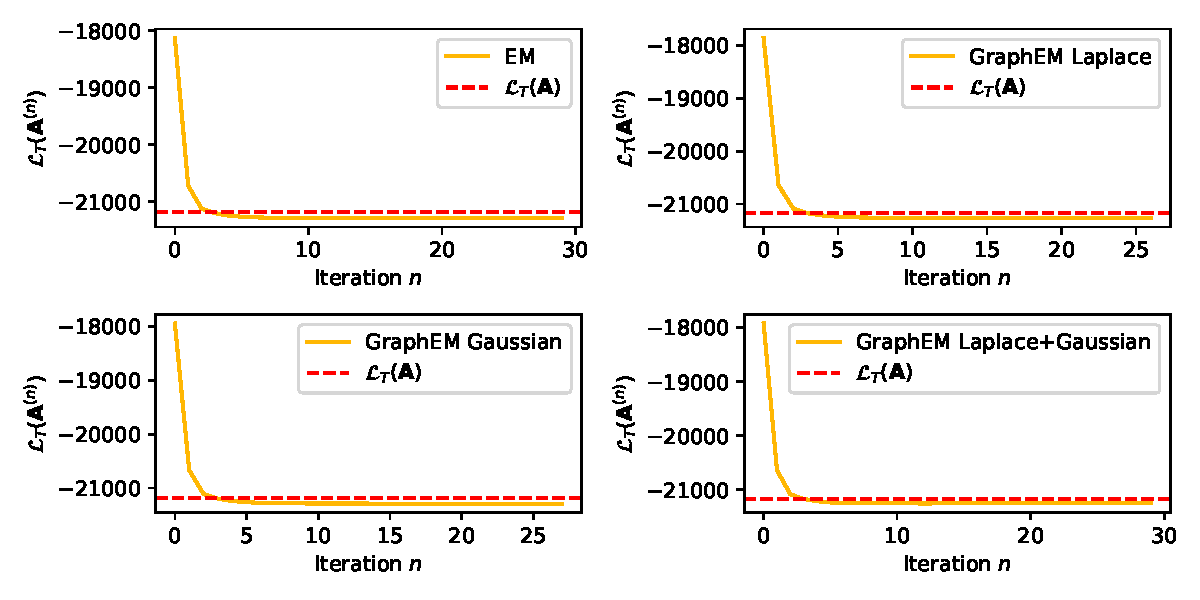
\includegraphics[width=0.75\linewidth]{fig/block diagonal/neg_log_likelihood.pdf}
    \caption{不同正则化方法下,分块对角图的负对数似然收敛曲线。}
    \label{fig: neg log likelihood}
\end{figure}

图~\ref{fig: neg log likelihood} 展示了分块对角图在不同正则方法下的负对数似然收敛情况。从图中可以看出,所有 EM 系列方法的收敛值均低于真实参数对应的负对数似然值,进一步验证了其估计效果的有效性。
\end{frame}


\begin{frame}
\begin{figure}[tb]
    \centering
    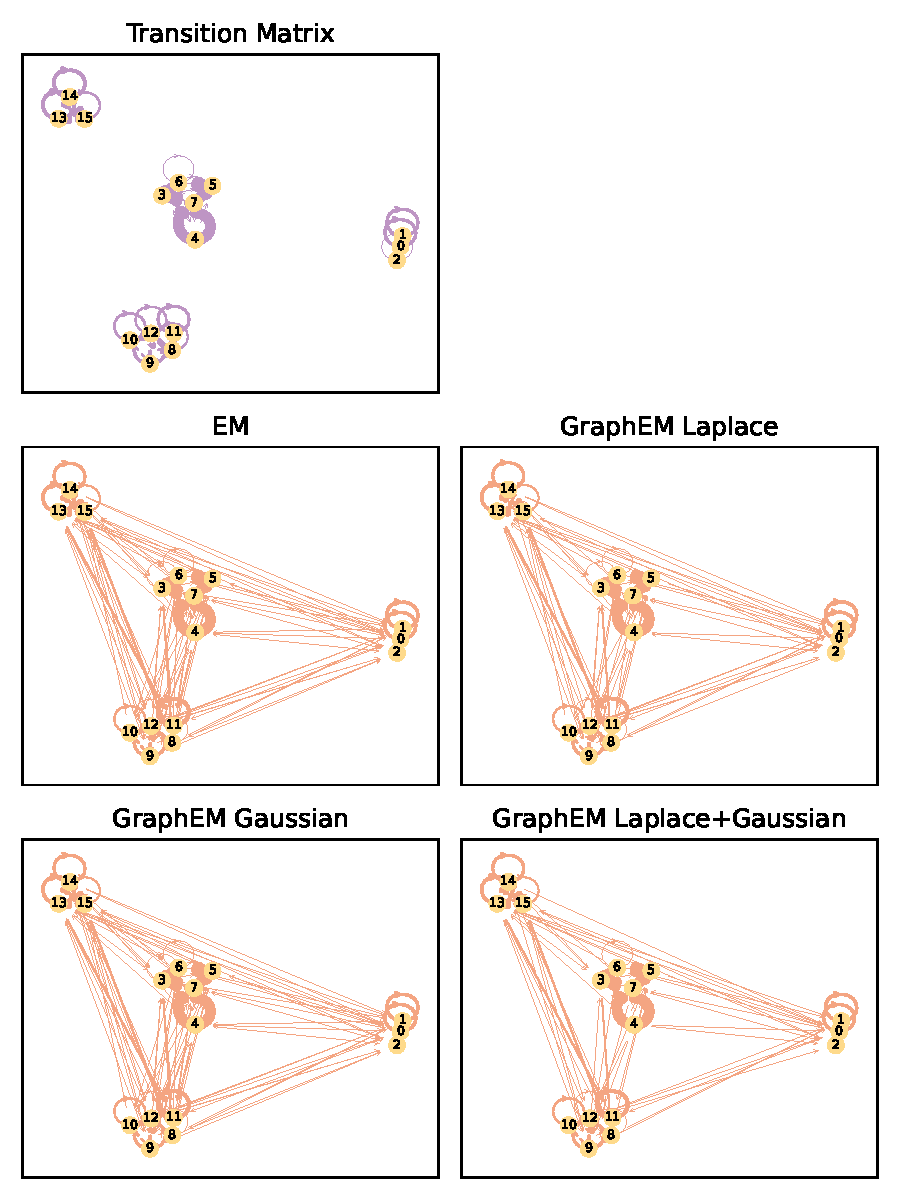
\includegraphics[width=0.3\linewidth]{fig/block diagonal/graphs_for_true_and_EM.pdf}
    \caption{分块对角图的真实转移矩阵与估计矩阵对比图。}
    \label{fig: graph comparison}
\end{figure}

为了进行更细致的对比,图~\ref{fig: graph comparison} 可视化展示了分块对角图的真实转移矩阵与估计转移矩阵。结果显示,GraphEM 的 Laplace 与 Laplace+Gaussian 方法所得估计最接近真实值,非对角块间联系更少,更好地保留了块对角结构。
\end{frame}


\begin{frame}{结论}
本文研究了 GraphEM 算法在线性高斯状态空间模型(LGSSM)参数估计中的应用。GraphEM 是一种新颖的算法,它将先验知识整合进期望最大化(EM)框架中。通过引入图推理与正则化技术,我们对原始 GraphEM 方法进行了扩展,使其能够处理更广泛的图结构与正则化策略,包括 Laplace、Gaussian 及混合 Laplace+Gaussian 先验。
\vspace{8pt}
\pause

一个具有前景的结果是,GraphEM 框架能够集成多种正则项。Laplace 与 Gaussian 先验的组合实现了两者优势的叠加,而不引入额外的优化开销。这一特性为未来的研究开辟了新方向:通过累积多样化的正则项,可以在不增加计算复杂度的前提下,迭代地逼近最优解。
\vspace{8pt}
\pause

未来的研究方向包括发展自适应正则化策略,根据观测数据与图结构动态调整 Laplace 与 Gaussian 先验的权重。此外,进一步研究 GraphEM 在其他图类型上的表现,如随机图、分层图与动态图,有助于验证其通用性。最后,将 GraphEM 应用于金融、气候建模与社交网络分析等实际问题中,有望展示其在参数估计中的实用价值与潜在影响。
\end{frame}


%------------------------------------------------

\begin{frame}
\Huge{\centerline{The End}}
\end{frame}

\begin{frame}
\bibliography{main}
\bibliographystyle{alpha} 
\end{frame}

%----------------------------------------------------------------------------------------

\end{document} 
